\documentclass[a4, 11pt]{article}

\usepackage{microtype}
%\usepackage[T1]{fontenc} % dejar solo para html
\usepackage[latin1]{inputenc}

\textwidth = 6.5 in 
\textheight = 9 in 
\oddsidemargin = 0.0 in
\evensidemargin = 0.0 in 
\topmargin = 0.0 in
\headheight = 0.0 in 
\headsep = 0.0 in
\parindent = 0.3in
\parskip=10pt
 
\usepackage{graphicx}
\graphicspath{{Fotos/}}

\usepackage{amsmath}
\usepackage{amsfonts}
\usepackage{harmony}
\usepackage{enumerate}
\usepackage{enumitem}
\usepackage{bm}
\usepackage{upgreek}

%% ddphonism
% 
% (c) Celia Rubio Madrigal
%
%% This program can be redistributed and/or modified under the terms
%% of the LaTeX Project Public License Distributed from CTAN archives
%% in directory macros/latex/base/lppl.txt.
 
\NeedsTeXFormat{LaTeX2e}
\ProvidesPackage{ddphonism}
[2019/08/10 v0.2 Dodecaphonic diagrams: twelve-tone matrices, clock diagrams, etc.]

\RequirePackage{etoolbox}
\RequirePackage{xparse}
\RequirePackage{tikz}
\RequirePackage{xstring}
\RequirePackage{pgfkeys}


%%%%%%%%%%%%%%%%%%%%%%%%%%%%%%%%%%%%
% Matrices

\usetikzlibrary{matrix}

\ExplSyntaxOn
\DeclareExpandableDocumentCommand{\Evaluation}{m}{\int_eval:n {#1}}
\ExplSyntaxOff

\newcounter{Dsize}
\newcommand{\DsizeMake}[1]{%
	\setcounter{Dsize}{0}%
	\foreach \n in {#1}{%
		\stepcounter{Dsize}%
	}%
}

% Only with numbers.
\newcounter{Dfirst}
\newcommand{\DheadMake}[1]{%
	\setcounter{Dfirst}{-1}%
	\foreach \n in {#1}{%
		\ifnum\theDfirst=-1%
		\setcounter{Dfirst}{\n}%
		\fi%
	}%
}

% Only when DsizeMake is already done.
\newcounter{Dmod}
\newcommand{\Modulo}[1]{%
	\setcounter{Dmod}{#1}%
	\loop%
	\ifnum\theDmod>\Evaluation{\theDsize-1}%		
		\setcounter{Dmod}{\Evaluation{\theDmod-\theDsize}}%
		\repeat%
	\ifnum\theDmod<0%
		\setcounter{Dmod}{\Evaluation{\theDmod+\theDsize}}%
		\repeat%
	\theDmod%
}

\newif\ifdmatrixLines
\newif\ifdmatrixOutside
\newif\ifdmatrixInside
\newif\ifdmatrixV
\newif\ifdmatrixH
\newif\ifdmatrixTikz
\pgfkeys{
	/dmatrix/.is family
	, /dmatrix
	, default/.style = 
		{ lines = false
		, outside lines = false
		, inside lines = false
		, sep = 1
		, vsep = 1
		, hsep = 1
		, no tikz = false
		}
	, no tikz/.is if=dmatrixTikz
	, lines/.is if=dmatrixLines
	, outside lines/.is if=dmatrixOutside
	, inside lines/.is if=dmatrixInside
	, vlines/.is if=dmatrixV
	, hlines/.is if=dmatrixH
	, sep/.estore in=\dmatrixSep
	, vsep/.estore in=\dmatrixVsep
	, hsep/.estore in=\dmatrixHsep
}

\newcommand{\DLOH}{%
	\draw (0.05*\dmatrixSep*\dmatrixHsep,0) --%
	(\theDsize*\dmatrixSep*\dmatrixHsep+0.05*\dmatrixSep*\dmatrixHsep,0);%
	\draw (0.05*\dmatrixSep*\dmatrixHsep,-\theDsize*0.5*\dmatrixSep*\dmatrixVsep) -- %
	(\theDsize*\dmatrixSep*\dmatrixHsep+0.05*\dmatrixSep*\dmatrixHsep,-\theDsize*0.5*\dmatrixSep*\dmatrixVsep);%
}

\newcommand{\DLOV}{%
	\draw (0.05*\dmatrixSep*\dmatrixHsep,0) -- %
	(0.05*\dmatrixSep*\dmatrixHsep,-\theDsize*0.5*\dmatrixSep*\dmatrixVsep);%
	\draw (\theDsize*\dmatrixSep*\dmatrixHsep+0.05*\dmatrixSep*\dmatrixHsep,0) -- %
	(\theDsize*\dmatrixSep*\dmatrixHsep+0.05*\dmatrixSep*\dmatrixHsep,-\theDsize*0.5*\dmatrixSep*\dmatrixVsep);
}

\newcommand{\DLIH}{%
	\draw (0.05*\dmatrixSep*\dmatrixHsep,-\xD*0.5*\dmatrixSep*\dmatrixVsep) -- %
	(\theDsize*\dmatrixSep*\dmatrixHsep+0.05*\dmatrixSep*\dmatrixHsep,-\xD*0.5*\dmatrixSep*\dmatrixVsep);%
}

\newcommand{\DLIV}{%
	\draw (\xD*\dmatrixSep*\dmatrixHsep+0.05*\dmatrixSep*\dmatrixHsep,0) -- %
	(\xD*\dmatrixSep*\dmatrixHsep+0.05*\dmatrixSep*\dmatrixHsep,-\theDsize*0.5*\dmatrixSep*\dmatrixVsep);%
}

\newcommand{\dmatrix}[2][]{%
	\DsizeMake{#2}%
	\DheadMake{#2}%
	%
	\pgfkeys{/dmatrix, default, #1}%
	%
	\ifdmatrixTikz\else%
	\begin{tikzpicture}%
	\fi%
	\foreach [count=\nj] \j in {#2} {%
		\foreach [count=\ni] \i in {#2} {%
			\draw node at 
			( \ni*\dmatrixSep*\dmatrixHsep-0.5*\dmatrixSep*\dmatrixHsep
			, -\nj*\dmatrixSep*\dmatrixVsep/2+0.25*\dmatrixSep*\dmatrixVsep) {%
				\Modulo{\Evaluation{\i-\j+\theDfirst}}%
			};%
		}%
	}%
	\foreach \xD in {1,...,\Evaluation{\theDsize-1}} {%
		\ifdmatrixLines
		\DLOH\DLOV\DLIH\DLIV
		\fi
		\ifdmatrixOutside
		\DLOH\DLOV
		\fi
		\ifdmatrixInside
		\DLIH\DLIV
		\fi
		\ifdmatrixH
		\DLOH\DLIH
		\fi
		\ifdmatrixV
		\DLOV\DLIV
		\fi
	}%
%
\ifdmatrixTikz\else%
\end{tikzpicture}%
\fi%
}


%%%%%%%%%%%%%%%%%%%%%%%%%%%%%%%%%%%%
% Diagrams

\usetikzlibrary{shapes,arrows,decorations.markings,shapes.misc}

\tikzstyle ddiagramArrow=[decoration=
		{markings,mark=at position 0.25 with
			{\arrow[scale=1.25,>=triangle 45]{>}}},
	postaction={decorate}]

\tikzstyle{ddiagram}=[minimum height=0pt,inner sep=0pt,outer sep=0pt,scale=0.65]

\newif\ifddiagramTikz
\pgfkeys{
	/ddiagram/.is family
	, /ddiagram
	, default/.style = 
		{ name =\empty%
		, up =\empty%
		, no tikz = false
		}
	, no tikz/.is if=ddiagramTikz
	, name/.estore in=\ddiagramName
	, up/.estore in=\ddiagramUp
}

\newcounter{Dprev}
\newcommand{\Dvar}{}
\newcommand{\ddiagram}[2][]{%
	\DsizeMake{#2}%
	\DheadMake{#2}%
	%
	\pgfkeys{/ddiagram, default, #1}%
	%
	\ifdefequal{\ddiagramUp}{\empty}%
	{\renewcommand{\Dvar}{\theDfirst}}% if empty
	{\renewcommand{\Dvar}{\ddiagramUp}}% if not empty
	%
	\ifddiagramTikz\else%
	\begin{tikzpicture}[ddiagram,rotate=360*\Dvar/\theDsize]%
	\fi%
	\foreach \x in {0,...,\Evaluation{\theDsize-1}} {%
		\node at (90-360*\x/\theDsize:2) {\x};%
		\node (\x) at (90-360*\x/\theDsize:1.6) {};%
	};%
	%
	\setcounter{Dprev}{-1}%
	\foreach \x in {#2}{%
		\ifnum \theDprev=\theDfirst%
		\draw [style=ddiagramArrow] (\theDprev) -- (\x);%
		\else \ifnum \theDprev=-1%
		\else%
		\draw (\theDprev) -- (\x);%
		\fi\fi%
		\setcounter{Dprev}{\x}%
	};%
	\draw (\theDprev) -- (\theDfirst);%
	%
	\ifdefequal{\ddiagramName}{\empty}%
	{}% if empty
	{\node at (0,0) [circle,fill=white] {\ddiagramName};}% if not empty
	\ifddiagramTikz\else%
	\end{tikzpicture}%
	\fi%
}


%%%%%%%%%%%%%%%%%%%%%%%%%%%%%%%%%%%%
% Dihedral diagrams

\tikzstyle ddihedralArrow=[decoration=
		{markings,mark=at position 1 with {\arrow[scale=1.5,>=angle 60]{>}}},
	postaction={decorate}]

\tikzstyle{ddihedral}=[inner sep=0,minimum height=18pt]

\newif\ifddihedralTikz
\pgfkeys{
	/ddihedral/.is family, /ddihedral,
	default/.style = {t = 0, c = 0, s = 0, v = 0, no tikz=false},
	no tikz/.is if=ddihedralTikz,
	t/.estore in = \ddihedralT,
	c/.estore in = \ddihedralC,
	s/.estore in = \ddihedralS,
	v/.estore in = \ddihedralV,
}

\newif\ifdarrowsTikz
\pgfkeys{
	/darrows/.is family, /darrows,
	default/.style = {no tikz=false},
	no tikz/.is if=darrowsTikz,
}
\newcommand{\darrows}[2][]{%
	\DsizeMake{#2}%
	%
	\pgfkeys{/darrows, default, #1}%
	%
	\ifdarrowsTikz\else%
	\begin{tikzpicture}%
	\fi%
	\draw foreach \x in {0,...,\Evaluation{\theDsize-1}} {%
		(90-360*\x/\theDsize:2.5) node[circle] (\x) {}%
	};%
	\foreach \x [count=\y] in {#2} {%
		\draw [style=ddihedralArrow] (90-360*\Evaluation{\y-1}/\theDsize:1.25) -- (\x);%
	};%
	\ifdarrowsTikz\else%
	\end{tikzpicture}%
	\fi%
}

\newcommand\ddihedral[2][]{%
	\DsizeMake{#2}%
	%
	\pgfkeys{/ddihedral, default, #1}%
	%
	\ifddihedralTikz\else%
	\begin{tikzpicture}[ddihedral]%
	\fi%
	\draw foreach \x in {0,...,\Evaluation{\theDsize-1}} {%
		(\Evaluation{(90+\ddihedralT*360/\theDsize)+(2*\ddihedralS-1)*\x*360/\theDsize}:2.5)%
		node[very thin,circle,draw] (\x) {\x}%
	};%
	%
	\draw foreach \x in {0,...,\Evaluation{\theDsize-1}} {%
		(\Evaluation{(90-\ddihedralC*360/\theDsize)+(2*\ddihedralV-1)*\x*360/\theDsize}:1.25)%
		node[very thin,circle,draw] {\x}%
	};%
	%
	\darrows[no tikz]{#2}%
	%
	\node at (0,0) [very thin,draw,circle, fill=white] {%
		\ifnum\ddihedralV=0%
		\ifnum\ddihedralC=0%
		\ifnum\ddihedralS=0%
		\ifnum\ddihedralT=0%
		P%
		\fi\fi\fi%
		\else V\fi%
		\ifnum\ddihedralC=0%
		\else C$^{\ddihedralC}$\fi%
		\ifnum\ddihedralS=0%
		\else S\fi%
		\ifnum\ddihedralT=0%
		\else T$^{\ddihedralT}$\fi%
	};%
	\ifddihedralTikz\else%
	\end{tikzpicture}%
	\fi%
}


%%%%%%%%%%%%%%%%%%%%%%%%%%%%%%%%%%%%
% Rows

\pgfkeys{
	/drow/.is family, /drow,
	default/.style = {sep=\arraycolsep},
	sep/.estore in = \drowSep,
}

\long\def\addto#1#2{\expandafter\def\expandafter#1\expandafter{#1#2}}
\newcounter{myDDcntr}
\newlength{\Dvarr}
	
\newcommand{\drow}[2][]{%
	\DsizeMake{#2}%
	%
	\pgfkeys{/drow, default, #1}%
	\setlength{\Dvarr}{\arraycolsep}
	\setlength{\arraycolsep}{\drowSep}
	%
	\ifnum\theDsize=0%
	\ensuremath{\left(\right)}%
	\else\ifnum\theDsize=1%
	\ensuremath{%
		\left(\begin{array}{*{\theDsize}c}%
			0\\%
			#2\\%
		\end{array}\right)%
	}%
	\else%
	\def\TableDDdata{}%
	\setcounter{myDDcntr}{0}%
	\loop%
	\addto\TableDDdata{\themyDDcntr\stepcounter{myDDcntr} &}%
	\stepcounter{myDDcntr}%
	\ifnum\themyDDcntr<\Evaluation{\theDsize-1}%
	\repeat%
	\addto\TableDDdata{\themyDDcntr \\}%
	\setcounter{myDDcntr}{0}%
	%
	\ensuremath{%
		\left(\begin{array}{*{\theDsize}c}%
			\TableDDdata%
			\StrSubstitute{#2}{,}{&}\\%
		\end{array}\right)%
	}%
	\fi\fi%
	\setlength{\arraycolsep}{\Dvarr}
}


%%%%%%%%%%%%%%%%%%%%%%%%%%%%%%%%%%%%
% Chord diagram

\newcommand{\dchords}[2][]{
	\DsizeMake{#2}
	\begin{tikzpicture}[ddihedral]
	\foreach[count=\nx] \x in {#2} {
		\node (\x) at (90+360/\theDsize-\nx*360/\theDsize:2) {};
	}
	\foreach \x in {#2} {
		\ifnum\Evaluation{\x-\theDsize/2}<0
		\ifodd\theDsize
		\draw (\x) -- (\Evaluation{\x+\theDsize/2-1});
		\else
		\draw (\x) -- (\Evaluation{\x-\theDsize/2});
		\fi\fi
	}
	\foreach[count=\nx] \x in {#2} {
		\node[very thin,circle,draw,fill=white] (\x) at (90+360/\theDsize-\nx*360/\theDsize:2) {\x};
	}
	\end{tikzpicture}
}

\usetikzlibrary{
	knots,
	hobby,
	decorations.pathreplacing,
	shapes.geometric,
	calc
}

\endinput


%% End of file `ddphonism.sty'.

\usepackage{multicol}
\PassOptionsToPackage{hyphens}{url}
\usepackage{hyperref}

% Complex \xxx for making notes of things to do.  Use \xxx{...} for general
% notes, and \xxx[who]{...} if you want to blame someone in particular.
% Puts text in brackets and in bold font, and normally adds a marginpar
% with the text ``xxx'' so that it is easy to find.  On the other hand, if
% the comment is in a minipage, figure, or caption, the xxx goes in the text,
% because marginpars are not possible in these situations.
{\makeatletter
 \gdef\xxxmark{%
   \expandafter\ifx\csname @mpargs\endcsname\relax % in minipage?
     \expandafter\ifx\csname @captype\endcsname\relax % in figure/caption?
       \marginpar{xxx}% not in a caption or minipage, can use marginpar
     \else
       xxx % notice trailing space
     \fi
   \else
     xxx % notice trailing space
   \fi}
 \gdef\xxx{\@ifnextchar[\xxx@lab\xxx@nolab}
 \long\gdef\xxx@lab[#1]#2{{\bf [\xxxmark #2 ---{\sc #1}]}}
 \long\gdef\xxx@nolab#1{{\bf [\xxxmark #1]}}
 % This turns them off:
% \long\gdef\xxx@lab[#1]#2{}\long\gdef\xxx@nolab#1{}%
}

\renewcommand\refname{Bibliograf�a}
\renewcommand\figurename{Figura}

\title{Serialismo y matem�ticas - III}
\author{Celia Rubio Madrigal}
\date{Noviembre de 2019}

\begin{document}
\maketitle

\section{Introducci�n}
	
 
	Este art�culo es el tercero y �ltimo de la colecci�n {\it Serialismo y matem�ticas}. Las m�sicas serialistas son aquellas que permiten construir castillos con un solo grano de arena: una serie particular, una permutaci�n de notas, din�micas o timbres. La serie se coloca en la obra secuencialmente, siempre igual o con alguna modificaci�n que la adorne. Y es que para esta m�sica,  la serie es el ladrillo y las matem�ticas son la pintura con la que decorarlos, ya que las transformaciones que se le puede aplicar a una serie forman preciosas estructuras matem�ticas enmarcadas en la Teor�a de Grupos.
	
	En el primer art�culo~\cite{celia1} nos centramos en el dodecafonismo, en sus or�genes y en comentar una de sus obras. En el segundo art�culo~\cite{celia2} ampliamos las definiciones dodecaf�nicas para encontrar el grupo di�drico, y descubrimos la historia de los disc�pulos de Schoenberg y del serialismo integral.
	
	Esta tercera entrega est� destinada al lector m�s ducho en las matem�ticas; se notar� en el lenguaje y en la exposici�n de las ideas. En ella proporcionaremos herramientas matem�ticas relacionadas con \textbf{acciones}, \textbf{�rbitas} y \textbf{estabilizadores} de Teor�a de Grupos (\hyperref[ch:acciones]{secci�n 2}), para despu�s contar de dos maneras distintas el \textbf{n�mero de espectros seriales}, que son el n�mero de �rbitas del grupo de transformaciones sobre las series, que un compositor puede utilizar en sus obras (\hyperref[ch:espectros]{secci�n 3}); en concreto, con las transformaciones $\{I,\ T,\ R\}$ (\hyperref[s:itr]{3.1}) y $\{S,\ T,\ V,\ C\}$ (\hyperref[s:stvc]{3.2}). Y de esta manera habremos hecho un recorrido a fondo por el serialismo y habremos explorado sus posibilidades musicales y matem�ticas.
	
	\chapter{MÁS HERRAMIENTAS MATEMÁTICAS}\label{ch:acciones}
	\section{Acciones de grupos sobre conjuntos}
		Dado un grupo (G, $*$) y un conjunto X, la \emph{acción} de (G, $*$) sobre X es una función $\phi$ que asocia un elemento $g \in$ G y un elemento $x \in$ X -- el par ($g$, $x$) -- a otro elemento $g\cdot x$ que también pertenece a X \cite{armstrong}. $\ \ \phi :(g,x) \to g\cdot x$
	
		La acción $\phi$, expresada mediante la operación ($\cdot$), debe cumplir dos condiciones:
		\begin{enumerate}
			\item{Para todo $x\in$ X, $e\cdot x=x$, siendo $e$ el elemento neutro del grupo.}
		
			\item{Para todo $x\in$ X y para todo par $g,h\in$ G, se debe cumplir que $(g*h)\cdot x=g\cdot (h\cdot x)$. La primera operación ($*$) es la interna del grupo G, y la segunda operación ($\cdot$) es la acción.}
		\end{enumerate}
		Como ya se ha visto en el apartado \ref{grupoD}, las funciones \{S,T,V,C\} forman el grupo diédrico $\text{D}_{n}\times\text{D}_{n}$, con $n$ la longitud de la serie. Se podrá definir entonces la acción $\phi$ de este grupo sobre el conjunto de permutaciones de orden $n$, tal que $\phi(\Psi,\ \sigma)=\Psi\circ\sigma=\Psi(\sigma)=\tau$, con $\Psi\in\text{D}_{n}\times\text{D}_{n}$ y $\sigma,\tau\in\text{S}_n$.
		
		De igual manera, se puede definir el grupo que forman solamente I y R, que servirá más adelante. Como son dos reflexiones, forman el conocido grupo de Klein -- a partir de ahora denotado por $\Xi$, con elementos Id, I, R e IR.

	\section{Órbitas y estabilizadores}	
		Dada una acción de (G, $*$) sobre X, la \emph{órbita} de un determinado elemento $x_0\in$ X es el subconjunto de elementos $x$ de X que pueden ser alcanzados desde $x_0$ mediante algún $g_0\in$ G. Es decir, todos los $x$ para los que existe un $g_0$ que al actuar sobre $x_0$ da $x$. Trivialmente, $x_0\in Orb(x_0)$ ya que $e\cdot x_0=x_0$.
		\[Orb(x_0)=\{x\in X :\ \exists \ g_0\in \text{G},\ g_0\cdot x_0 =x\}\]
	
		Por ejemplo, dada una permutación $\sigma$, todas las permutaciones a las que se llega desde $\sigma$ mediante algún $\Psi\in\text{D}_{n}\times\text{D}_{n}$ -- que son las transformaciones de series del apartado \ref{ciclico} -- conforman la órbita de $\sigma$. Por definición, las series a las que se puede llegar desde una serie original conforman su espectro serial, por lo que \textbf{la órbita es en realidad el espectro serial}.
	
		Para el mismo $x_0$ se define su \emph{estabilizador} como el conjunto de elementos $g\in$ G que fijan $x_0$, es decir, que mandan $x_0$ a sí mismo. Mientras que una órbita es un subconjunto de X, un estabilizador es un subgrupo de G. Trivialmente, $e\in Stab(x) \ \forall x\in$ X, porque el elemento identidad fija cualquier otro elemento por definición.
		\[Stab(x_0)=\{g\in \text{G}\ :\ g\cdot x_0 =x_0 \}\]
	
		Si cada $g\in$ G llevara a $x_0$ a un $x$ distinto, el número de elementos de $Orb(x_0)$ sería igual al número de elementos de G. Sin embargo, si un elemento $g_0\in$ G fija $x_0$, entonces no dará nuevos elementos en la órbita de $x$. Por tanto, el tamaño de la órbita disminuye. De hecho,  el teorema de Órbita--Estabilizador dice que el tamaño de una órbita ($|Orb(x_0)|$) será el tamaño de G ($|$G$|$) entre el número de elementos que fijan $x_0$; es decir, el tamaño de su estabilizador ($|Stab(x_0)|$). Además, es cierto para todo $x\in$ X.
		\[|Orb(x)|=\frac{|\text{G}|}{|Stab(x)|}\text{, o lo que es lo mismo, }|\text{G}|=|Orb(x)||Stab(x)|\]
		
		\def\arraystretch{1.5}
		Este teorema implica que los tamaños de cada órbita y cada estabilizador son divisores del tamaño del grupo. Por ejemplo, como el tamaño del grupo $\Xi$ es 4, cualquier estabilizador y cualquier órbita tendrán tamaño 1, 2 o 4. En concreto, como Id está siempre en el estabilizador, para  todo $\sigma$ será de una de estas formas:
		\[\begin{matrix}|Stab|=1&&&\{\text{Id}\}&\\\hline|Stab|=2&&\{\text{Id, R}\}&\{\text{Id, I}\}&\{\text{Id, RI}\}\}\\\hline|Stab|=4&&&\{\text{Id, R, I, RI}\}&\\\end{matrix}\]
		
		\def\arraystretch{1}
		Una serie $\sigma$ sin simetrías tendrá una serie distinta para cada una de sus transformaciones. Por tanto, su órbita será \{$\sigma$, R($\sigma$), I($\sigma$), RI($\sigma$)\} y su estabilizador será solamente \{Id\}. Cumple entonces el teorema: $4\cdot 1 = 4$.
	
	\section{El lema de Burnside}
		\label{burnside}
		Las órbitas, que son subconjuntos de X, forman una \emph{partición} de X. Esto significa que son subconjuntos disjuntos: ningún $x$ puede estar en dos órbitas distintas. Interesa entonces saber cuántos subconjuntos hay; es decir, el número de órbitas ($\#Orb$). El lema de Burnside\footnote{Aunque Burnside demostró este lema en una ocasión, citó a Frobenius como su autor. Sin embargo, Cauchy era conocedor del lema décadas antes. Para no confundirlo con otros lemas que sí son de Burnside, a veces se le llama \emph{el lema que no es de Burnside.}} afirma que se pueden calcular así:
		\[\#Orb=\frac{1}{|\text{G}|}\sum_{x\in\text{X}}|\text{Stab}(x)|\]	
		Se prueba de esta forma: por el teorema de Órbita--Estabilizador, $|\text{Stab}(x)|=\frac{|\text{G}|}{|Orb(x)|}$, por lo que la parte derecha se puede expresar así:
		\[\frac{1}{|\text{G}|}\sum_{x\in\text{X}}|\text{Stab}(x)|=
		\frac{1}{|\text{G}|}\sum_{x\in\text{X}}\frac{|\text{G}|}{|Orb(x)|}=
		\sum_{x\in\text{X}}\frac{1}{|Orb(x)|}\]

		Como las órbitas forman una partición de X, la suma sobre todo el conjunto X puede ser dividida en sumas separadas para cada órbita. Además, si por cada elemento de una órbita se suma el inverso del número de elementos de la órbita, esa suma dará uno. Solo queda ahora sumar uno por cada órbita.
		\[\sum_{x\in\text{X}}\frac{1}{|Orb(x)|}=\sum_{\text{O}\in\text{Órbitas}}\left(\sum_{x\in\text{O}}\frac{1}{|\text{O}|}\right)=\sum_{\text{O}\in\text{Órbitas}}1=\#Orb \qed\]	
	
		Este lema permite calcular el número de posibles espectros seriales distintos, ya que el espectro de una serie es igual al espectro de sus series transformadas. Un compositor serialista debe entonces escoger no una serie original, sino el espectro con el que construir la obra. O, más bien, si escoge una serie original está escogiendo el mismo material que si escogiera otra serie de ese mismo espectro.%
	\section{Conteo de espectros seriales}\label{ch:espectros}
	\subsection{Espectros de las funciones $\{I,\ T,\ R\}$}
		\label{s:itr}
		Es interesante conocer el n�mero de espectros seriales distintos que un compositor puede escoger. Al fin y al cabo, es irrelevante qu� serie se escoge como la original dentro de su espectro serial, ya que produce el mismo material compositivo que cualquiera de su mismo espectro.
		
		Para calcular el n�mero de espectros seriales se redefinir�n las funciones transformativas para una longitud serial arbitraria, $n$, que ser� mayor que 2. Para $n=0,\ 1$ y 2 se realizar� el c�lculo en el apartado \ref{s:trivcase}.
	
		Adem�s, como las transposiciones siempre son distintas entre s�, siempre pertenecen al mismo espectro. Se tomar�n a partir de ahora todas ellas como equivalentes, de manera que solo se necesita hacer el c�lculo para $\{I,\ R\}$.
		
		Al calcular con permutaciones se trabajar� m�dulo $n$. La retrogradaci�n sigue siendo $R(\sigma(m))=\sigma(-1-m)$. La inversi�n ser� $I(\sigma(m))=-\sigma(m)$, omitiendo la transposici�n habitual, ya que se toman las series transpuestas como equivalentes. De esta forma $-\sigma(m)+2\sigma(0)\equiv-\sigma(m)$. La retrogradaci�n invertida es, por tanto, la composici�n de ambas: $RI(\sigma(m))={I}\circ{R}(\sigma(m))={I}\left({R}(\sigma(m))\right)=-\sigma(-1-m)$.			
		
		La retrogradaci�n, la inversi�n y la composici�n de ambas cumplen que al aplicarlas dos veces se vuelve a la serie original. En teor�a de grupos se dice que tienen \textit{orden 2}. Entonces $\{Id,\ I,\ R,\ IR\}$ forma el ya mencionado grupo de Klein ($\Xi$), donde $RI$ $\equiv$ $IR$, ya que estamos tomando las series transpuestas como equivalentes. 
		
		En general, un grupo de Klein es el formado por cuatro elementos donde cada elemento es inverso de s� mismo. El grupo de Klein, llamado as� en honor al matem�tico alem�n Felix Klein, es el grupo $\mathbb{Z}/(2)\times\mathbb{Z}/(2)$, producto directo de dos grupos c�clicos de orden 2.
		
		Por el lema de Burnside:
		\[\#\mbox{Espectros}=\frac{1}{|\mathbb{Z}/(2)\times\mathbb{Z}/(2)|}\sum_{\sigma\in{S}_n}|{Stab}(\sigma)|=\frac{1}{4}\sum_{\sigma\in{S}_n}|{Stab}(\sigma)|\]
		
		Es decir, se deben calcular para cada posible serie $\sigma\in{S}_n$ cu�ntas funciones transformativas lo dejan igual o equivalente bajo transposici�n.
		
		Como los estabilizadores son subgrupos, por el teorema de Lagrange su tama�o debe ser divisor del tama�o del grupo total. Entonces se pueden agrupar los estabilizadores por sus tama�os: 1, 2 o 4, y as� calcular $\sum|{Stab}(\sigma)|$ agrupando todas las permutaciones con igual tama�o de estabilizador. Si $\#\sigma_i$ es el n�mero de permutaciones cuyos estabilizadores tienen tama�o $i$:		
		\[\sum_{\sigma\in{S}_n}|{Stab}(\sigma)|=1\cdot(\#\sigma_1)+2\cdot(\#\sigma_2)+4\cdot(\#\sigma_4)\]
	
		Primero, se ha de ver que una permutaci�n nunca va a ser igual ni equivalente mediante transposiciones a su inversa.

%		\begin{align*}
%		-\sigma(m)&\equiv\sigma(m)\Longleftrightarrow\\
%		0&\equiv2\sigma(m)\Longleftrightarrow\\
%		n&\equiv2\sigma(m)\Longleftrightarrow\\
%		\frac{n}{2}&\equiv\sigma(m)
%		\end{align*}
\begin{center}
		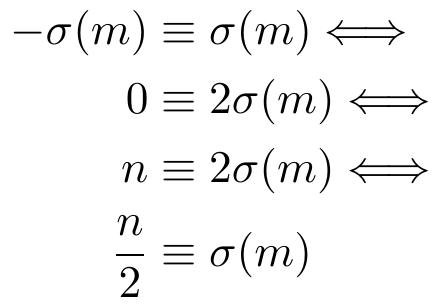
\includegraphics{Serialismo-matematicas-diagrama-2}
\end{center}
		
		As�, $\sigma(m)$ ser�a constante para todo $m\in \mathbb{Z} / (n)$, lo cual es imposible. Esto implica que ninguna permutaci�n va a tener a $I$ en su estabilizador, por lo que $\#\sigma_4=0$. Queda entonces calcular cu�ntas permutaciones son equivalentes a su retrogradaci�n y cu�ntas a su retrogradaci�n inversa. La suma de ambas dar� $\#\sigma_2$.
	
	\subsubsection[Elementos estables mediante $R$]{Elementos estables mediante ${R}$}
		Las permutaciones que coinciden con alguna transposici�n de su retrogradaci�n cumplen, para $\gamma$ constante:
		
		\hspace*{8.5\bigskipamount} $\gamma+\sigma(m) = {R}(m) = \sigma(-1-m)$
		
		Aplic�ndolo a $(-1-m)$:
		$\gamma+\sigma(-1-m) = \sigma(m)$
		
		De ambas ecuaciones: $\quad\gamma=\sigma(-1-m)-\sigma(m)=\sigma(m)-\sigma(-1-m)$
		
		$2\sigma(m)\equiv2\sigma(-1-m)\implies2\sigma(m)-2\sigma(-1-m)\equiv0$
		
		$2\sigma(m)-2\sigma(-1-m)=n \implies \sigma(m)-\sigma(-1-m)=\frac{n}{2}$
		
		Entonces $n$ debe ser par. Cuando $n$ es impar este tipo de permutaciones no existe. Adem�s, cumplen que sus elementos sim�tricos se distancian entre s� un intervalo de $\frac{n}{2}$ unidades: son series con simetr�a par.
		\[\gamma=\sigma(m)-\sigma(-1-m)=\frac{n}{2}\]
		
		En una serie de longitud $n$, existen $\frac{n}{2}$ intervalos que miden $\frac{n}{2}$. Como no importa por cu�l de ellos comience la serie, ya que las transportaciones son equivalentes, se fija el primero de los intervalos. Quedan los otros $\frac{n}{2}-1$ intervalos por escoger, as� que el n�mero de series con simetr�a par cuenta las permutaciones de $\frac{n}{2}-1$ intervalos y las dos posibles posiciones de cada intervalo \textemdash creciente y decreciente~\cite{reiner}\textemdash. Por ello, el n�mero de series con simetr�a par es de:
		
		\[2! \cdot \left(\frac{n}{2}-1\right)! = 2\left(\frac{n-2}{2}\right)!=(n-2)(n-4)\ldots=(n-2)!!\]
		
		Por definici�n, si $n$ es par $n!!=n(n-2)(n-4)\ldots4\cdot2$ y si $n$ es impar $n!!=n(n-2)(n-4)\ldots3\cdot1$.

	\subsubsection[Elementos estables mediante $RI$]{Elementos estables mediante ${RI}$}
		Las permutaciones que coinciden con alguna transposici�n de su retrogradaci�n inversa cumplen, para un $\gamma$ constante:
		\[\sigma(m)={RI}(\sigma(m))+\gamma=-\sigma(-1-m)+\gamma\]
		\[\gamma=\sigma(m)+\sigma(-1-m)\]
		
		Sus elementos sim�tricos suman una cantidad constante: son series con simetr�a impar. Tal y como se ha hecho en el apartado anterior, se puede fijar una de las notas, ya que las transportaciones son equivalentes. Si $n$ es impar, la nota central es $\sigma(\frac{n-1}{2})$, que es igual a $\sigma(-1-\frac{n-1}{2})$. Por tanto, $\gamma=2\cdot\sigma(\frac{n-1}{2})$. Si se escoge esta nota para ser fijada a 0, entonces $\gamma=2\cdot0=0$. Es decir, $\gamma$ puede ser fijada a 0 sin p�rdida de generalidad.
		
		Para el resto de notas, $\sigma(m)=-\sigma(-1-m)$. Ya escogida la nota central, permite $n-1$ posibilidades para $\sigma(0)$. Ya escogidas la nota central, la primera y su sim�trica, permiten $n-3$ posibilidades para $\sigma(1)$, y as� sucesivamente hasta llegar a la nota anterior a la central, que es $\frac{n-3}{2}$. Por ello, para $n$ impar, el n�mero de series con simetr�a impar es de:	
		\[(n-1)(n-3)\ldots(n-2\cdot\frac{n-5}{2}-1)(n-2\cdot\frac{n-3}{2}-1)=\]
		\[=(n-1)(n-3)\ldots(n-(n-5)-1)(n-(n-3)-1)=\]
		\[=(n-1)(n-3)\ldots4\cdot2=(n-1)!!\]
		
		Si $n$ es par, $\sigma(m)\neq\sigma(-1-m)\ \forall m\in \mathbb{Z} / (n)$, ya que no hay elemento central. Sea ahora $\gamma=2k$ un n�mero par. Como $2k\leq n$ y las permutaciones son suprayectivas, para alg�n $m$ se cumple que $\sigma(m)=k$. Se tiene entonces $k+\sigma(-1-m)=2k\implies\sigma(-1-m)=k=\sigma(m)$. Como esto es una contradicci�n, $\gamma$ debe ser impar.
		
		Fijando, por ejemplo, $\sigma(0)=0$, se tienen $\frac{n}{2}$ posibilidades para $\sigma(-1-m)$, es decir, solamente las posibilidades para las que $\gamma$ es impar. Para $\sigma(1)$ hay $(n-2)$ posibilidades, y ahora su sim�trico ya viene determinado por el $\gamma$ escogido. Para $\sigma(2)$ hay $(n-4)$, y as� sucesivamente~\cite{reiner}. Por tanto, para $n$ par, el n�mero de series con simetr�a impar es de: 
		\[\frac{n}{2}\cdot(n-2)(n-4)\ldots(n-2\cdot\frac{n-4}{2})(n-2\cdot\frac{n-2}{2})=\]
		\[=\frac{n}{2}\cdot(n-2)(n-4)\ldots(n-(n-4))(n-(n-2))=\]
		\[=\frac{n}{2}\cdot(n-2)(n-4)\ldots4\cdot2=\frac{n}{2}\cdot(n-2)!!\]
			
	\subsubsection*{Suma completa}
		Como ya se ha podido observar, el n�mero de espectros seriales var�a seg�n la paridad de la longitud de las series.		
		\def\arraystretch{1.5}
		\[\begin{array}{c|c|c|c|c}
		&\{Id,\ I\}&\{Id,\ R\}&\{Id,\ RI\}&\#\sigma_2\\\hline
		n\mbox{ impar}&0&0&(n-1)!!&(n-1)!!\\\hline
		n\mbox{ par}&0&(n-2)!!&\frac{n}{2}\cdot(n-2)!!&\frac{1}{2}(n+2)(n-2)!!\\
		\end{array}\]
		\def\arraystretch{1}
		
		Una vez se tiene $\#\sigma_2$, solo falta calcular $\#\sigma_1$. Como las permutaciones contadas $\#\sigma$ son todas las de ${S}_n$ exceptuando las transportaciones, $\#\sigma=\frac{\#\mbox{S}_n}{n}=\frac{n!}{n}=(n-1)!$. Por otro lado, $\#\sigma_1 +\#\sigma_2=\#\sigma$. Entonces $\#\sigma_1=(n-1)!-\#\sigma_2$.
		
		Recuperando la f�rmula del apartado \ref{s:itr}:
		
		\[\#\mbox{Espectros}=
		\frac{1}{4}\left(\#\sigma_1+2\cdot(\#\sigma_2)\right)=
		\frac{(n-1)!+\#\sigma_2}{4}\]
		
		Para $n$ impar:
		\[\frac{(n-1)!+(n-1)!!}{4}=\frac{(n-1)!!\cdot\left((n-2)!!+1\right)}{4}\]
		
		Para $n$ par:
		\[\frac{(n-1)!+\left(\frac{1}{2}(n+2)(n-2)!!\right)}{4}=\frac{2(n-1)!+(n+2)(n-2)!!}{8}\]
		
		Para $n=12$, es decir, para el dodecafonismo, la �ltima f�rmula proporciona el dato de 9985920 espectros seriales a escoger por el compositor.
		
		Como ejemplo perteneciente al serialismo integral, podemos numerar las din�micas del 0 al 6:
		\[\{ppp,\ pp,\ p,\ m\!f,\ f,\ f\!\!f,\ f\!\!f\!\!f\} \equiv \{0,\ 1,\ 2,\ 3,\ 4,\ 5,\ 6\} = \mathbb{Z} / (7)\]
		
		As�, con la f�rmula para $n$ impar, se obtiene que hay 192 espectros seriales con series de longitud 7.
	
	
	\subsection{Espectros del grupo ${D_n\times D_n}$}\label{s:stvc}
	
		Este apartado es una explicaci�n detallada del art�culo \cite{polygons} y aplicada al caso musical. La secuencia de n�meros dada por las f�rmulas que obtendremos se encuentra en la OEIS: \url{https://oeis.org/A000940}.
	
		\begin{figure}[h]
			\begin{center}
%			\ddiagram[no numbers, no arrow]{4,5,7,1,6,3,8,2,11,0,9,10}
			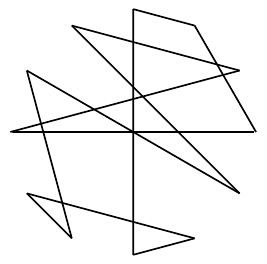
\includegraphics{Serialismo-matematicas-diagrama-3}
			\end{center}
		\end{figure}
		Ahora calcularemos los espectros formados mediante todas las transformaciones del grupo generado por $\{S,\ T,\ V,\ C\}$; es decir, por ${D}_{n}\times {D}_{n}$. Volviendo a la representaci�n mediante diagramas de reloj, el problema es equivalente a averiguar cu�ntos diagramas distintos, sin n�meros ni flechas, se pueden dibujar. La flecha indica lo transformado por $V$ y $C$, mientras que los n�meros indican lo transformado por $S$ y $T$. Un diagrama sin estos dos elementos representa entonces todo un espectro serial. ¿Cu�ntos diagramas esencialmente distintos hay? De nuevo, por el lema de Burnside:
		\[\#\mbox{Espectros}=\frac{1}{|{D}_{n}\times{D}_{n}|}\sum_{\sigma\in{S}_n}|{Stab}(\sigma)|=\frac{1}{2n\cdot2n}\sum_{\sigma\in{S}_n}|{Stab}(\sigma)|\]
		
		En vez de expresar el sumatorio como ``para cada $\sigma$, el n�mero de $\Psi$ que fijan $\sigma$'', se puede expresar como ``para cada $\Psi$, el n�mero de $\sigma$ fijados por $\Psi$''. La f�rmula queda de esta manera:
		
		\[\#\mbox{Espectros}=\frac{1}{4n^2}\sum_{\Psi\in{D}_{n}\times{D}_{n}}{Fij}(\Psi)\] 
		
		Ahora hay que averiguar para cada elemento de ${D}_{n}\times{D}_{n}$ cu�ntas series estabiliza. Por ejemplo, trivialmente no hay permutaciones estables mediante $C$ y $V$ solamente.
		
		
		\subsubsection[Elementos estables mediante $T$]{Elementos estables mediante ${T}$}
		
		Los elementos estables mediante $T^{k}$ son a los que, tras aplicar una rotaci�n de $\uptheta_{k}=\frac{2\pi k}{n}$, para $1\leq k\leq n$, quedan igual. Por tanto, los sumandos que aportan a la suma total son $\sum\limits_{k=1}^{n}{Fij}(\uptheta_{k})$.
		
		Por otro lado, si $1\leq p,q\leq n$ y $gcd(p,n)=gcd(q,n)$ entonces ${Fij}(\uptheta_p)={Fij}(\uptheta_q)$, ya que por el lema de B�zout lo que genera la rotaci�n $\uptheta_p$ es igual a lo que genera la rotaci�n $\uptheta_{{gcd}(p,n)}$. Esto permite que se puedan agrupar los sumandos con igual m�ximo com�n divisor con respecto a $n$. Es decir, $\sum\limits_{k=1}^{n}{Fij}(\uptheta_{k})=\sum\limits_{d|n}\left(\mathcal{C}\cdot{Fij}(\uptheta_d)\right)$, con $d$ divisor de $n$.
		Por ejemplo, si $n=6$:
		\begin{align*}
			&{Fij}(\uptheta_{1})+{Fij}(\uptheta_{2})+{Fij}(\uptheta_{3})+{Fij}(\uptheta_{4})+{Fij}(\uptheta_{5})+{Fij}(\uptheta_{6})=\\
			&{Fij}(\uptheta_{1})+{Fij}(\uptheta_{2})+{Fij}(\uptheta_{3})+{Fij}(\uptheta_{2})+{Fij}(\uptheta_{1})+{Fij}(\uptheta_{6})=\\
			&2\cdot{Fij}(\uptheta_{1})+2\cdot{Fij}(\uptheta_{2})+1\cdot{Fij}(\uptheta_{3})+1\cdot{Fij}(\uptheta_{6})
		\end{align*}
		
		
		Ahora queremos encontrar el coeficiente $\mathcal{C}$ de ${Fij}(\uptheta_d)$, es decir, el n�mero de $k\leq n$ con igual m�ximo com�n divisor $d$. Pero que $k\leq n$ y $gcd(k,n)=d$ es equivalente a que $ \frac{k}{d}\leq\frac{n}{d}$ y $gcd\left(\frac{k}{d},\frac{n}{d}\right)=1$. Por tanto, el n�mero de $k$ con m�ximo comun divisor $d$ es $\varphi\left(\frac{n}{d}\right)$. La funci�n $\varphi(x)$ se llama la funci�n \textit{phi} de Euler, y muestra precisamente la cantidad de n�meros menores que �l y coprimos con �l. Entonces $\sum\limits_{{k}=1}^{n}{Fij}(\uptheta_{{k}})=\sum\limits_{d|n}\left(\varphi(\frac{n}{d})\cdot{Fij}(\uptheta_d)\right)$.
		
		Para calcular ${Fij}(\uptheta_d)$ hay que analizar c�mo se construyen los diagramas invariantes respecto a una rotaci�n. Estos diagramas deben tener varios \textit{ciclos} iguales entre s� \textemdash para que queden invariantes al rotarlos\textemdash~pero cada uno desde un punto distinto: desde cada m�ltiplo de $d$. El n�mero de ciclos es, por tanto, $\frac{n}{d}$.
		
		Al construir uno de estos diagramas, se escoge la primera nota entre las $n$. Despu�s se escoge la segunda, pero no se pueden escoger los v�rtices m�ltiplos de $d$ (de los que hay $\frac{n}{d}$), ya que van a ser el comienzo de los sucesivos ciclos. Hay entonces $n-\frac{n}{d}$ posibilidades. Despu�s se escoge la tercera, pero sin escoger los m�ltiplos de $d$ ni los m�ltiplos de $d\ +$ la segunda posici�n. Hay $n - 2\cdot\frac{n}{d}$ posibilidades, y as� sucesivamente hasta terminar el primer ciclo:
		\[n\left(n-\frac{n}{d}\right)\left(n-\frac{2n}{d}\right)\cdots\left(n-\frac{(d-1)n}{d}\right)=\] 
		\[=n^d\left(1-\frac{1}{d}\right)\left(1-\frac{2}{d}\right)\cdots\left(1-\frac{d-1}{d}\right)=\]
		\[=n^d\left(\frac{d-1}{d}\right)\left(\frac{d-2}{d}\right)\cdots\left(\frac{1}{d}\right)=n^d\cdot\frac{(d-1)!}{d^{d-1}}\cdot\frac{d}{d}=\left(\frac{n}{d}\right)^d\cdot d!\]
		
		Por ejemplo, si $d=2$ y $n=8$, supongamos que escogemos el punto 0$^{(0)}$ como el primero. Despu�s, si cogi�ramos alguno de los puntos 0$^{(*)}$ luego no podr�amos tener simetr�a al rotarlo un �ngulo de $\uptheta_2$. Entonces hay que escoger alguno de los 1$^{(*)}$. Supongamos que es 1$^{(1)}$. En este ejemplo nuestro \textit{ciclo} quedar�a de la siguiente manera:
		
%		\begin{figure}[h]
			\begin{center}
%				\begin{tikzpicture}
%			\node [draw,circle,inner sep=0,minimum height=2cm] at (0,0) {};
%			\foreach\y in {0,1,2,3} {
%				\foreach\x in {0,1} {
%					\draw[thin] (90-45*\x-90*\y:0.85) -- (90-45*\x-90*\y:1.35) node[fill=white,inner sep=0pt] {\x$^{(\y)}$};
%				}
%			}
%			\draw (90:1) -- (-45:1);
%			\end{tikzpicture}
			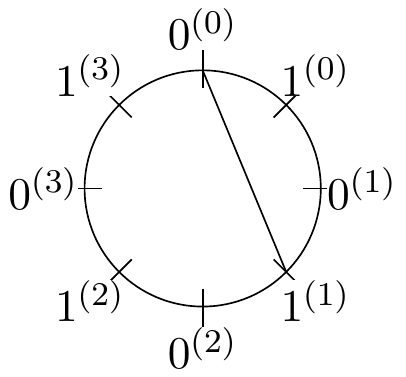
\includegraphics{Serialismo-matematicas-diagrama-4}
			\end{center}
%		\end{figure}
		
		Para escoger el segundo ciclo, su primera nota debe caer en el conjunto de v�rtices m�ltiplos de $d$ \textemdash de los que hay $\frac{n}{d}$. En el ejemplo ser�an los 0$^{(*)}$. Sin embargo, no podr�a ser cualquier m�ltiplo, ya que si se escoge uno con posici�n no coprima, el pol�gono se cerrar�a antes de tiempo sin pasar por todos los v�rtices. Entonces hay que escoger entre los v�rtices coprimos, de los que hay $\varphi\left(\frac{n}{d}\right)$. Tras esto el pol�gono est� totalmente determinado, y se puede formar de $\sum\limits_{d|n}\left(\varphi^2(\frac{n}{d})\cdot\left(\frac{n}{d}\right)^d\cdot d!\right)$ maneras.
		
		En nuestro ejemplo, si escogemos el siguiente comienzo del ciclo como el 0$^{(2)}$, como 2 no es coprimo con $\frac{n}{d}=4$, quedar�a de esta manera:
		
		\begin{center}
%			\begin{multicols}{2}
%				\begin{tikzpicture}
%				\node [draw,circle,inner sep=0,minimum height=2cm] at (0,0) {};
%				\foreach\y in {0,1,2,3} {
%					\foreach\x in {0,1} {
%						\draw[thin] (90-45*\x-90*\y:0.85) -- (90-45*\x-90*\y:1.35) node[fill=white,inner sep=0pt] {\x$^{(\y)}$};
%					}
%				}
%				\draw (90:1) -- (-45:1) -- (-90:1);
%				\end{tikzpicture}
%				
%				\begin{tikzpicture}
%				\node [draw,circle,inner sep=0,minimum height=2cm] at (0,0) {};
%				\foreach\y in {0,1,2,3} {
%					\foreach\x in {0,1} {
%						\draw[thin] (90-45*\x-90*\y:0.85) -- (90-45*\x-90*\y:1.35) node[fill=white,inner sep=0pt] {\x$^{(\y)}$};
%					}
%				}
%				\draw (90:1) -- (-45:1) -- (-90:1);
%				\draw[rotate=-180] (90:1) -- (-45:1) -- (-90:1);
%				\end{tikzpicture}
%			\end{multicols}
		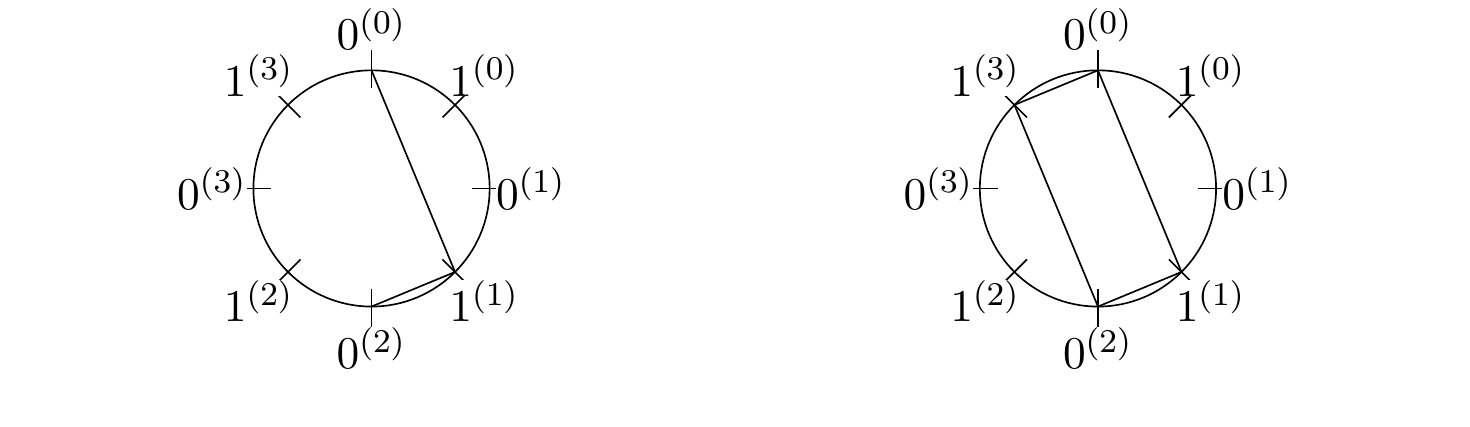
\includegraphics{Serialismo-matematicas-diagrama-5}
		\end{center}

		Efectivamente, el diagrama se cierra antes de pasar por todos los v�rtices. En cambio, si escogemos 0$^{(1)}$:
%		\begin{multicols}{4}			
%			\begin{tikzpicture}
%			\node [draw,circle,inner sep=0,minimum height=2cm] at (0,0) {};
%			\foreach\y in {0,1,2,3} {
%				\foreach\x in {0,1} {
%					\draw[thin] (90-45*\x-90*\y:0.85) -- (90-45*\x-90*\y:1.35) node[fill=white,inner sep=0pt] {\x$^{(\y)}$};
%				}
%			}
%		\draw (90:1) -- (-45:1) -- (0:1);
%%		\draw[rotate=-90] (90:1) -- (-45:1) -- (0:1);
%%		\draw[rotate=180] (90:1) -- (-45:1) -- (0:1);
%%		\draw[rotate=90] (90:1) -- (-45:1) -- (0:1);
%			\end{tikzpicture}
%			
%			\begin{tikzpicture}
%			\node [draw,circle,inner sep=0,minimum height=2cm] at (0,0) {};
%			\foreach\y in {0,1,2,3} {
%				\foreach\x in {0,1} {
%					\draw[thin] (90-45*\x-90*\y:0.85) -- (90-45*\x-90*\y:1.35) node[fill=white,inner sep=0pt] {\x$^{(\y)}$};
%				}
%			}
%			\draw (90:1) -- (-45:1) -- (0:1);
%			\draw[rotate=-90] (90:1) -- (-45:1) -- (0:1);
%%			\draw[rotate=180] (90:1) -- (-45:1) -- (0:1);
%%			\draw[rotate=90] (90:1) -- (-45:1) -- (0:1);
%			\end{tikzpicture}
%			
%			\begin{tikzpicture}
%			\node [draw,circle,inner sep=0,minimum height=2cm] at (0,0) {};
%			\foreach\y in {0,1,2,3} {
%				\foreach\x in {0,1} {
%					\draw[thin] (90-45*\x-90*\y:0.85) -- (90-45*\x-90*\y:1.35) node[fill=white,inner sep=0pt] {\x$^{(\y)}$};
%				}
%			}
%			\draw (90:1) -- (-45:1) -- (0:1);
%			\draw[rotate=-90] (90:1) -- (-45:1) -- (0:1);
%			\draw[rotate=180] (90:1) -- (-45:1) -- (0:1);
%%			\draw[rotate=90] (90:1) -- (-45:1) -- (0:1);
%			\end{tikzpicture}
%			
%			\begin{tikzpicture}
%			\node [draw,circle,inner sep=0,minimum height=2cm] at (0,0) {};
%			\foreach\y in {0,1,2,3} {
%				\foreach\x in {0,1} {
%					\draw[thin] (90-45*\x-90*\y:0.85) -- (90-45*\x-90*\y:1.35) node[fill=white,inner sep=0pt] {\x$^{(\y)}$};
%				}
%			}
%			\draw (90:1) -- (-45:1) -- (0:1);
%			\draw[rotate=-90] (90:1) -- (-45:1) -- (0:1);
%			\draw[rotate=180] (90:1) -- (-45:1) -- (0:1);
%			\draw[rotate=90] (90:1) -- (-45:1) -- (0:1);
%			\end{tikzpicture}
%		\end{multicols}
\begin{center}
	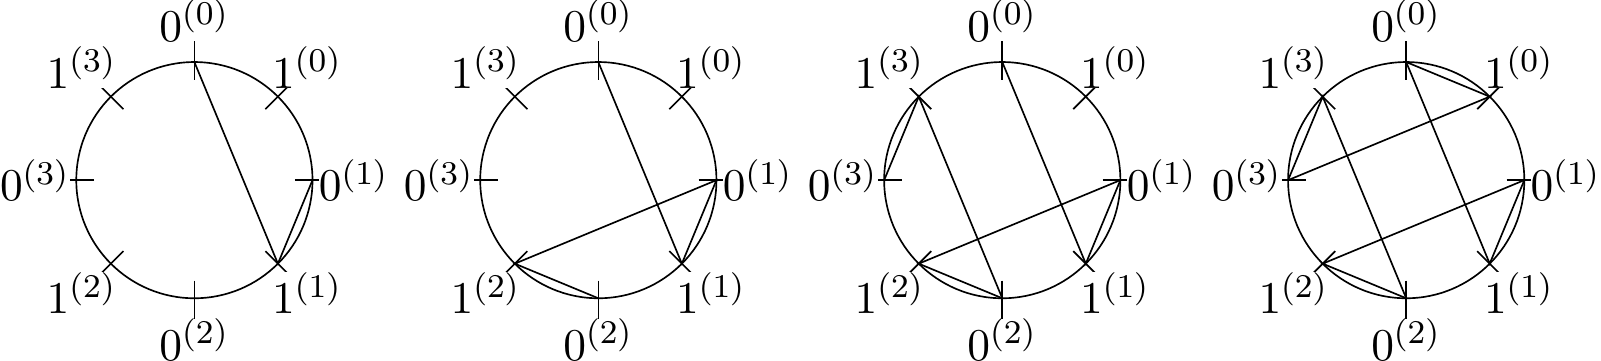
\includegraphics{Serialismo-matematicas-diagrama-6}
\end{center}
	
		Y con 0$^{(3)}$:
%		\begin{multicols}{4}			
%			\begin{tikzpicture}
%			\node [draw,circle,inner sep=0,minimum height=2cm] at (0,0) {};
%			\foreach\y in {0,1,2,3} {
%				\foreach\x in {0,1} {
%					\draw[thin] (90-45*\x-90*\y:0.85) -- (90-45*\x-90*\y:1.35) node[fill=white,inner sep=0pt] {\x$^{(\y)}$};
%				}
%			}
%			\draw (90:1) -- (-45:1) -- (180:1);
%	%		\draw[rotate=-90] (90:1) -- (-45:1) -- (180:1);
%	%		\draw[rotate=180] (90:1) -- (-45:1) -- (180:1);
%	%		\draw[rotate=90] (90:1) -- (-45:1) -- (180:1);
%			\end{tikzpicture}
%			
%			\begin{tikzpicture}
%			\node [draw,circle,inner sep=0,minimum height=2cm] at (0,0) {};
%			\foreach\y in {0,1,2,3} {
%				\foreach\x in {0,1} {
%					\draw[thin] (90-45*\x-90*\y:0.85) -- (90-45*\x-90*\y:1.35) node[fill=white,inner sep=0pt] {\x$^{(\y)}$};
%				}
%			}
%			\draw (90:1) -- (-45:1) -- (180:1);
%			\draw[rotate=-90] (90:1) -- (-45:1) -- (180:1);
%	%		\draw[rotate=180] (90:1) -- (-45:1) -- (180:1);
%	%		\draw[rotate=90] (90:1) -- (-45:1) -- (180:1);
%			\end{tikzpicture}
%			
%			\begin{tikzpicture}
%			\node [draw,circle,inner sep=0,minimum height=2cm] at (0,0) {};
%			\foreach\y in {0,1,2,3} {
%				\foreach\x in {0,1} {
%					\draw[thin] (90-45*\x-90*\y:0.85) -- (90-45*\x-90*\y:1.35) node[fill=white,inner sep=0pt] {\x$^{(\y)}$};
%				}
%			}
%			\draw (90:1) -- (-45:1) -- (180:1);
%			\draw[rotate=-90] (90:1) -- (-45:1) -- (180:1);
%			\draw[rotate=180] (90:1) -- (-45:1) -- (180:1);
%	%		\draw[rotate=90] (90:1) -- (-45:1) -- (180:1);
%			\end{tikzpicture}
%			
%			\begin{tikzpicture}
%			\node [draw,circle,inner sep=0,minimum height=2cm] at (0,0) {};
%			\foreach\y in {0,1,2,3} {
%				\foreach\x in {0,1} {
%					\draw[thin] (90-45*\x-90*\y:0.85) -- (90-45*\x-90*\y:1.35) node[fill=white,inner sep=0pt] {\x$^{(\y)}$};
%				}
%			}
%			\draw (90:1) -- (-45:1) -- (180:1);
%			\draw[rotate=-90] (90:1) -- (-45:1) -- (180:1);
%			\draw[rotate=180] (90:1) -- (-45:1) -- (180:1);
%			\draw[rotate=90] (90:1) -- (-45:1) -- (180:1);
%			\end{tikzpicture}
%		\end{multicols}
\begin{center}
		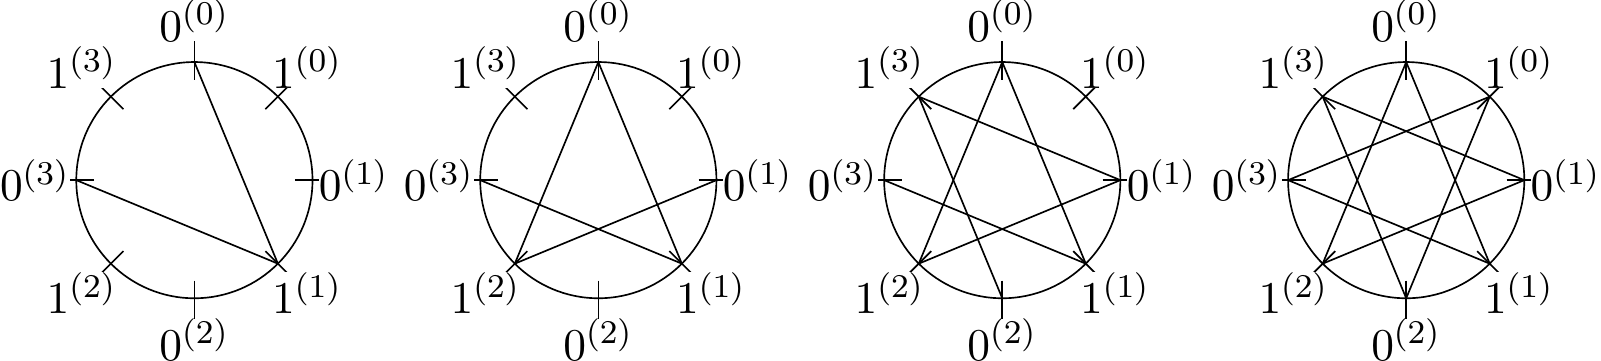
\includegraphics{Serialismo-matematicas-diagrama-7}
\end{center}
		
		Sea $d=3$ y $n=6$. Escogiendo el primer n�mero como 0$^{(0)}$, el segundo como 1$^{(0)}$ y el tercero como 2$^{(1)}$, no queda m�s remedio que escoger como comienzo del segundo ciclo el 0$^{(1)}$.
		
%	\begin{multicols}{3}
%		\begin{tikzpicture}
%		\node [draw,circle,inner sep=0,minimum height=2cm] at (0,0) {};
%		\foreach\y in {0,1} {
%			\foreach\x in {0,1,2} {
%				\draw[thin] (90-60*\x-180*\y:0.85) -- (90-60*\x-180*\y:1.35) node[fill=white,inner sep=0pt] {\x$^{(\y)}$};
%			}
%		}
%		\draw (90:1) -- (30:1) -- (150:1);
%		\end{tikzpicture}
%		
%		\begin{tikzpicture}
%		\node [draw,circle,inner sep=0,minimum height=2cm] at (0,0) {};
%		\foreach\y in {0,1} {
%			\foreach\x in {0,1,2} {
%				\draw[thin] (90-60*\x-180*\y:0.85) -- (90-60*\x-180*\y:1.35) node[fill=white,inner sep=0pt] {\x$^{(\y)}$};
%			}
%		}
%		\draw (90:1) -- (30:1) -- (150:1) -- (-90:1);
%		%		\draw[rotate=180] (90:1) -- (30:1) -- (150:1) -- (-90:1);
%		\end{tikzpicture}
%		
%		\begin{tikzpicture}
%		\node [draw,circle,inner sep=0,minimum height=2cm] at (0,0) {};
%		\foreach\y in {0,1} {
%			\foreach\x in {0,1,2} {
%				\draw[thin] (90-60*\x-180*\y:0.85) -- (90-60*\x-180*\y:1.35) node[fill=white,inner sep=0pt] {\x$^{(\y)}$};
%			}
%		}
%		\draw (90:1) -- (30:1) -- (150:1) -- (-90:1);
%		\draw[rotate=180] (90:1) -- (30:1) -- (150:1) -- (-90:1);
%		\end{tikzpicture}
%	\end{multicols}
\begin{center}
	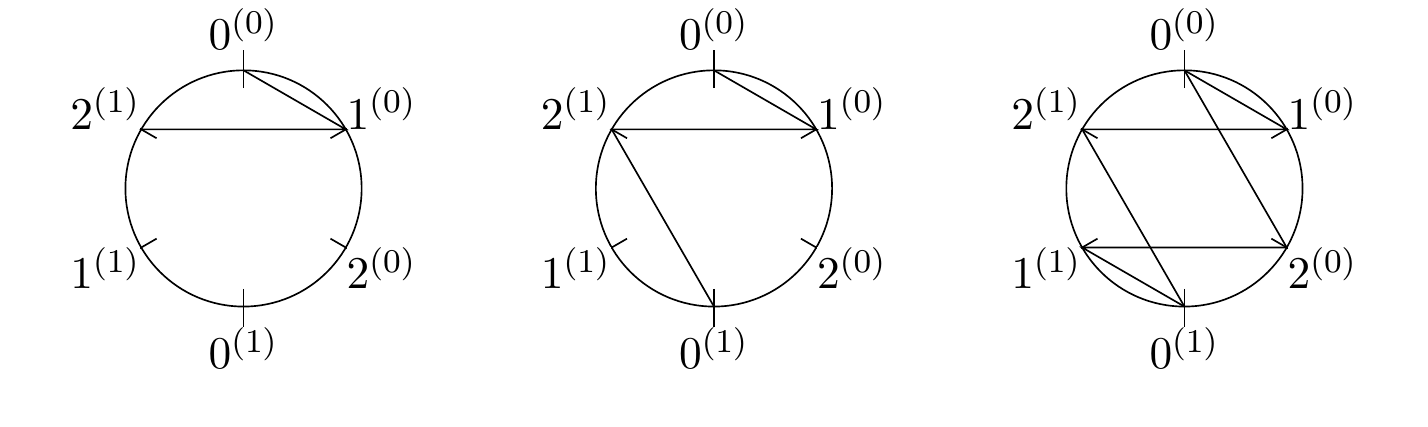
\includegraphics{Serialismo-matematicas-diagrama-8}
\end{center}

		Pero tambi�n podr�a aparecer este mismo comienzo con la parte final dada la vuelta, sim�trica, de esta manera: 0$^{(0)}$, 1$^{(0)}$, 2$^{(1)}$, 2$^{(0)}$, 1$^{(1)}$, 0$^{(1)}$. Esta construcci�n no est� incluida en lo descrito anteriormente, y sin embargo es invariante con respecto a T, V y C a la vez. 
		
%		\begin{multicols}{3}
%			\begin{tikzpicture}
%			\node [draw,circle,inner sep=0,minimum height=2cm] at (0,0) {};
%			\foreach\y in {0,1} {
%				\foreach\x in {0,1,2} {
%					\draw[thin] (90-60*\x-180*\y:0.85) -- (90-60*\x-180*\y:1.35) node[fill=white,inner sep=0pt] {\x$^{(\y)}$};
%				}
%			}
%			\draw (90:1) -- (30:1) -- (150:1);
%			\end{tikzpicture}
%			
%			\begin{tikzpicture}
%			\node [draw,circle,inner sep=0,minimum height=2cm] at (0,0) {};
%			\foreach\y in {0,1} {
%				\foreach\x in {0,1,2} {
%					\draw[thin] (90-60*\x-180*\y:0.85) -- (90-60*\x-180*\y:1.35) node[fill=white,inner sep=0pt] {\x$^{(\y)}$};
%				}
%			}
%			\draw (90:1) -- (30:1) -- (150:1);
%			\draw[rotate=180] (90:1) -- (30:1) -- (150:1);
%			\end{tikzpicture}
%			
%			\begin{tikzpicture}
%			\node [draw,circle,inner sep=0,minimum height=2cm] at (0,0) {};
%			\foreach\y in {0,1} {
%				\foreach\x in {0,1,2} {
%					\draw[thin] (90-60*\x-180*\y:0.85) -- (90-60*\x-180*\y:1.35) node[fill=white,inner sep=0pt] {\x$^{(\y)}$};
%				}
%			}
%			\draw (90:1) -- (30:1) -- (150:1);
%			\draw[rotate=180] (90:1) -- (30:1) -- (150:1);
%			\draw[] (-90:1) -- (90:1);
%			\draw[] (150:1) -- (-30:1);
%			\end{tikzpicture}
%		\end{multicols}
\begin{center}
		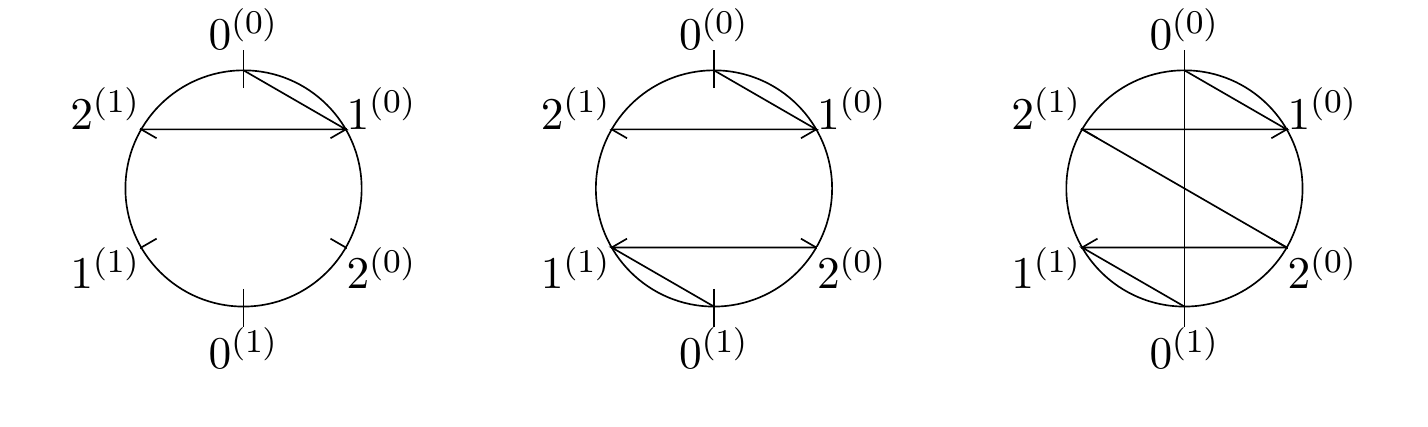
\includegraphics{Serialismo-matematicas-diagrama-9}
\end{center}
		
		Y es que con $n$ par, al rotar $\uptheta_{{n}/{2}}$ el diagrama, �ste puede llegar con la orientaci�n cambiada. Esto puede ocurrir cuando haya una diagonal; es decir, cuando entre dos notas haya un intervalo de $\frac{n}{2}$.
		
		\begin{center}
%		\begin{tikzpicture}[ddiagram]
%		\ddiagram[no tikz]{0,1,5,2,4,3}
%		
%		\draw[style=ddihedralArrow] (2.5,0) -- node[above=5pt] {T$^3$} (4,0);
%		
%		\ddiagram[no tikz, xshift=4cm]{3,4,2,5,1,0}
%		
%		\draw[style=ddihedralArrow,xshift=6cm] (2.5,0) -- node[above=5pt] {V} (4,0);
%		
%		\ddiagram[no tikz, xshift=8cm, arrow shift=1.25]{3,0,1,5,2,4}
%		
%		\draw[style=ddihedralArrow] (12.3,-2.5) -- (12.3,-3.25) -- node [fill=white] {C} (0,-3.25) -- (0,-2.5);
%		\end{tikzpicture}
		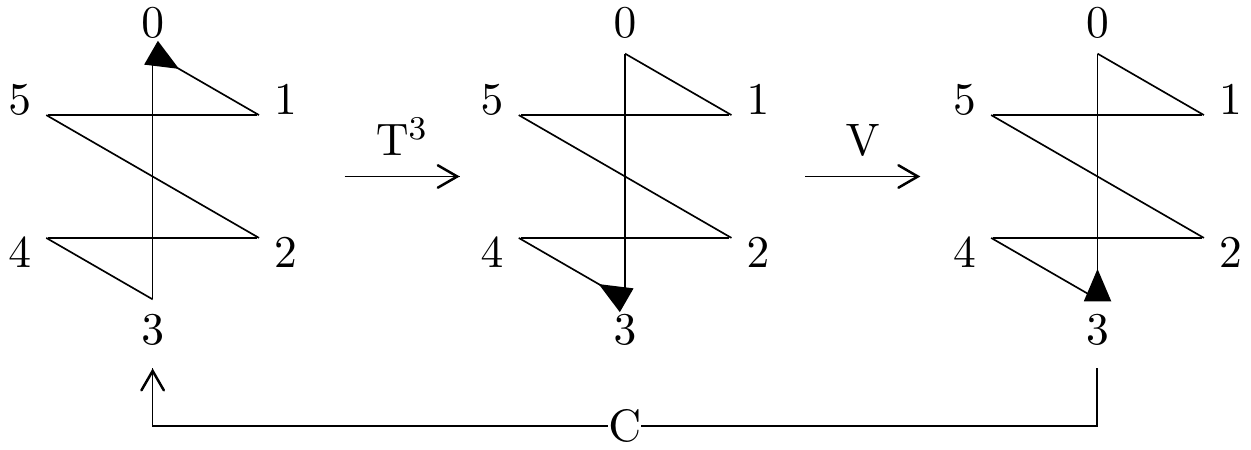
\includegraphics{Serialismo-matematicas-diagrama-10}
		\end{center}
		
		Se escoge el primer punto de entre $\frac{n}{2}$ posibilidades. No son $n$ ya que saldr�a la misma figura si se escoge el punto antipodal.
		Con una rotaci�n de $\uptheta_{{n}/{2}}$, el primer ciclo se escoge igual que antes, de $\left(\frac{n}{n/2}\right)^{\frac{n}{2}}\cdot \frac{n}{2}!=2^{\frac{n}{2}}\cdot \frac{n}{2}!$ maneras. Y con esto ya queda la figura determinada. Esto lleva a las $\frac{n}{2}\cdot2^{\frac{n}{2}}\cdot\frac{n}{2}!$ formas de dibujar un pol�gono con las caracter�sticas buscadas.
		
		\subsubsection[Elementos estables mediante $S$]{Elementos estables mediante ${S}$}
		
		Los elementos estables mediante $S$ son aquellos que quedan invariantes mediante reflexiones. En este punto se ha de separar por paridad de $n$. 
		
		Para $n$ impar, existen $n$ reflexiones para cada uno de los ejes de simetr�a que pasan por cada v�rtice. Despu�s, hay $n$ formas de escoger el primer v�rtice de la secuencia. Ahora hay $\frac{n-1}{2}$ parejas de v�rtices; se escoge los primeros miembros entre ellos de $2^{\frac{n-1}{2}}$ formas, tras lo cual �stos se ordenan de $\frac{n-1}{2}!$ formas. Esto da un resultado de  $n^2\cdot2^{\frac{n-1}{2}}\cdot\frac{n-1}{2}!$ pol�gonos invariantes.
		
		Para $n$ par se tienen dos simetr�as: con ejes que pasan por v�rtices y con ejes que pasan por lados. De manera similar a la anterior, se escoge el eje, el primer v�rtice, los primeros miembros de las parejas de v�rtices y se ordenan. Para las simetr�as con ejes que pasan por v�rtices, da un resultado de  $\frac{n^2}{2}\cdot2^{\frac{n}{2}}\cdot\left(\frac{n}{2}-1\right)!$. Para las simetr�as con ejes que pasan por lados, da un resultado de $\frac{n^2}{2}\cdot2^{\frac{n}{2}-1}\cdot\frac{n}{2}!$.
		
		\subsubsection*{Suma completa}
		
		En resumen, estos a continuaci�n son los numeradores $\sum%_{\Psi\in\mbox{D}_{n}\times\mbox{D}_{n}}
		{Fij}(\Psi)$. El resultado final del n�mero de diagramas posibles, o espectros seriales distintos, es dicho numerador entre $4n^2$, el tama�o del grupo. 	
		\def\arraystretch{1.5}
		\[\begin{array}{c||c}
		&\textbf{\textit{n} IMPAR}\\\hline\hline
		\mbox{Rotaci�n}&\sum\limits_{d|n}\left(\varphi^2(\frac{n}{d})\cdot\left(\frac{n}{d}\right)^d\cdot d!\right)\\\hline
		\mbox{Reflexi�n}&n^2\cdot2^{\frac{n-1}{2}}\cdot\frac{n-1}{2}!\\\hline
		&\sum\limits_{d|n}\left(\varphi^2(\frac{n}{d})\cdot\left(\frac{n}{d}\right)^d\cdot d!\right)+n^2\cdot2^{\frac{n-1}{2}}\cdot\frac{n-1}{2}!\\
		\end{array}\]
		
		\[\begin{array}{c||c}
		&\textbf{\textit{n} PAR}\\\hline\hline
		\mbox{Rotaci�n I}&\sum\limits_{d|n}\left(\varphi^2(\frac{n}{d})\cdot\left(\frac{n}{d}\right)^d\cdot d!\right)\\\hline
		\mbox{Rotaci�n II}&\frac{n}{2}\cdot2^{\frac{n}{2}}\cdot\frac{n}{2}!\\\hline
		\mbox{Reflexi�n v�rtices}&\frac{n^2}{2}\cdot2^{\frac{n}{2}}\cdot\left(\frac{n}{2}-1\right)!\\\hline
		\mbox{Reflexi�n lados}&\frac{n^2}{2}\cdot2^{\frac{n}{2}-1}\cdot\frac{n}{2}!\\\hline
		&\sum\limits_{d|n}\left(\varphi^2(\frac{n}{d})\cdot\left(\frac{n}{d}\right)^d\cdot d!\right)+\frac{n(n+6)}{4}\cdot2^{\frac{n}{2}}\cdot\frac{n}{2}!\\
		\end{array}\]
		\def\arraystretch{1}
		
	\subsection{Medefonismo, monofonismo y difonismo}
	\label{s:trivcase}
		Con $n=0$ se da el caso de medefonismo. El grupo sim�trico de orden 0 tiene $0!=1$ elemento. Por tanto, hay una sola posible serie, $\sigma$, que es la que no tiene ninguna nota. El medefonismo es com�nmente llamado silencio.
		
%		\[\sigma=\drow{}
%		\qquad\qquad\qquad
%		\begin{array}{l||r}
%		&\\
%		\hline
%		\hline
%		&\\
%		\hline
%		&
%		\end{array}\]
\begin{center}
			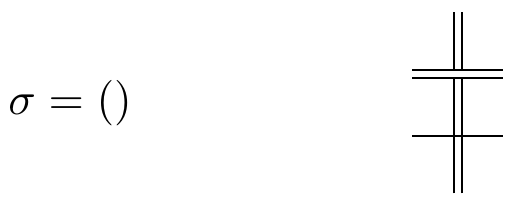
\includegraphics{Serialismo-matematicas-diagrama-11}
\end{center}
	
		Con $n=1$ se da el caso de monofonismo. Con solamente una posible nota, el grupo sim�trico de orden 1 tiene $1!=1$ elemento. Por tanto, hay una sola posible serie, $\sigma_0$, que es igual a su inversa, a su retrogradaci�n y a su retrogradaci�n inversa:
		
%		\[\sigma_0=\drow{0}
%		\qquad\qquad\qquad
%		\begin{array}{l|c|r}
%			&{I}_{0}&\\
%			\hline
%			{T}_{0}&0&{R}_{0}\\
%			\hline
%			&{IR}_{0}&\\
%			\hline
%			&{RI}_{0}&
%		\end{array}\]
\begin{center}
					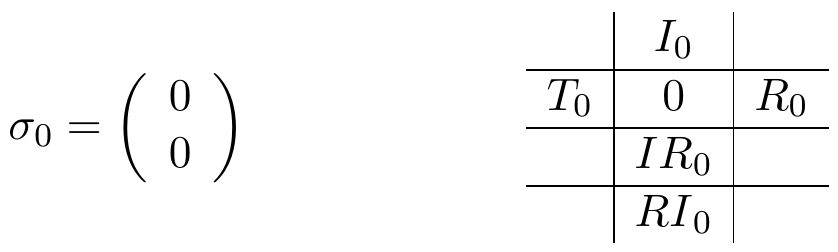
\includegraphics{Serialismo-matematicas-diagrama-12}
\end{center}
	
		Con $n=2$ se da el caso de difonismo. Tiene dos posibles notas, as� que su grupo sim�trico, el de orden 2, tiene $2!=2$ elementos. Por tanto, hay dos series distintas, $\sigma_0$ y $\sigma_1$. Se puede observar que ambas pertenecen al mismo espectro serial, dado que $\sigma_1={T}^1(\sigma_0)$. Adem�s, al igual que en el monofonismo, ambas coinciden con sus inversas, incumpliendo la regla general para $n>2$ probada en el apartado \ref{s:itr}.
		
%		\[\sigma_0=\drow{0,1}
%		\qquad\qquad
%		\begin{array}{l|cc|r}
%			&{I}_{0}&{I}_{1}&\\
%			\hline
%			{T}_{0}&0&1&{R}_{0}\\
%			{T}_{1}&1&0&{R}_{1}\\
%			\hline
%			&{IR}_{0}&{IR}_{1}&\\
%			\hline
%			&{RI}_{0}&{RI}_{1}&
%		\end{array}
%		\qquad\qquad
%		\sigma_1=\drow{1,0}\]
\begin{center}
					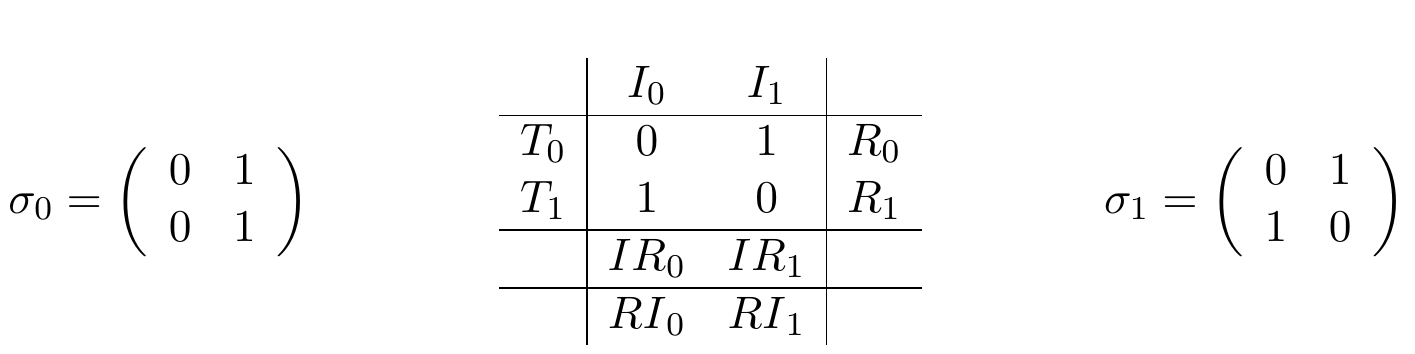
\includegraphics{Serialismo-matematicas-diagrama-13}
\end{center}
%
	
\bibliographystyle{plain}
\bibliography{Serialismo-matematicas-III.bib}
\end{document}
